\documentclass[conference]{IEEEtran}
\IEEEoverridecommandlockouts
% The preceding line is only needed to identify funding in the first footnote. If that is unneeded, please comment it out.
% Template version as of 6/27/2024

\usepackage{cite}
\usepackage{amsmath,amssymb,amsfonts}
\usepackage{algorithmic}
\usepackage{graphicx}
\usepackage{textcomp}
\usepackage{xcolor}
\usepackage{booktabs}
\usepackage{multirow}
\usepackage{url}
\usepackage{microtype}

\def\BibTeX{{\rm B\kern-.05em{\sc i\kern-.025em b}\kern-.08em
    T\kern-.1667em\lower.7ex\hbox{E}\kern-.125emX}}

\begin{document}

\title{DecisionSphere: A Scenario-Based Strategic Planning and Risk Evaluation Platform}

\author{\IEEEauthorblockN{P Naga Venkata Kushal}
\IEEEauthorblockA{\textit{School of Computer Science and Engineering} \\
\textit{Vellore Institute of Technology}\\
Vellore, Tamil Nadu, India \\
kushal.pnv2023@vitstudent.ac.in}
\and
\IEEEauthorblockN{P Manjunatha Kumar Tejas}
\IEEEauthorblockA{\textit{School of Computer Science and Engineering} \\
\textit{Vellore Institute of Technology}\\
Vellore, Tamil Nadu, India \\
tejas.pmk2023@vitstudent.ac.in}
\and
\IEEEauthorblockN{Jeswanth Reddy Sagabala}
\IEEEauthorblockA{\textit{School of Computer Science and Engineering} \\
\textit{Vellore Institute of Technology}\\
Vellore, Tamil Nadu, India \\
jeswanth.rs2023@vitstudent.ac.in}
\and
\IEEEauthorblockN{Dr. Suresh A}
\IEEEauthorblockA{\textit{School of Computer Science and Engineering} \\
\textit{Vellore Institute of Technology}\\
Vellore, Tamil Nadu, India \\
suresh.a@vit.ac.in}
}

\maketitle

\begin{abstract}
Strategic business interventions inherently trigger cascading cross-domain consequences across enterprise operations. However, contemporary enterprise decision support systems operate within isolated organizational silos: demand forecasting is restricted to sales, logistics delivery risk is isolated in fulfillment centers, and employee turnover is confined to human resources. Consequently, commercial initiatives such as promotional price cuts frequently induce unbuffered operational strains, resulting in carrier delivery delays, workforce overtime burnout, and catastrophic balance-sheet margin collapse. This paper presents DecisionSphere, an integrated decision intelligence platform that couples three independently trained, calibrated machine learning models across retail demand forecasting (Rossmann Store Sales), logistics delivery risk classification (DataCo Supply Chain), and employee attrition risk (IBM HR Analytics) into a unified 13-stage deterministic execution pipeline. These separate benchmark datasets do not originate from a single real-world firm and are coupled through explicit parameterized scenario assumptions (ASM-001 to ASM-008) without claiming universal causal relationships. Operational impacts are propagated across domains via deterministic coupling equations, feeding a transparent managerial accounting engine and a rule-grounded recommendation synthesizer. We enforce a strict six-tier epistemic hierarchy, preventing non-causal statistical inferences from being conflated with empirical fact or causal certainty. Evaluated on an authoritative enterprise scenario (+15.0\% demand shock, active promotional push, and 40.0\% mandatory overtime), DecisionSphere demonstrates how a commercial surge of +28,551.04 units generates +$26,710.78 in realized revenue yet triggers +$469,188.49 in carrier delay penalties and +$184,212.00 in labor disruption costs, collapsing net operating profit by -$642,716.18 and automatically triggering an objective restructuring rejection (REJECT\_RESTRUCTURE, Composite Risk Score 37.48). We substantiate our architecture through nine formal empirical experiments (EXP-001 through EXP-009), analyzing parameter-sensitive operational tipping points (such as the verified $+9.67\%$ unconstrained break-even threshold and $+18.4\%$ under relaxed logistics SLAs) and proving asymptotic Monte Carlo convergence across 200 stochastic perturbation runs.
\end{abstract}

\begin{IEEEkeywords}
Decision Intelligence, Strategic Planning, Cross-Domain Simulation, Demand Forecasting, Supply Chain Risk, Workforce Attrition, Probability Calibration, Explainable AI.
\end{IEEEkeywords}

\section{Introduction}

In contemporary enterprise management, operational decision-making relies heavily on predictive machine learning (ML) models. However, these analytical assets exist almost universally within isolated functional departments \cite{pratt2019decision}. Commercial marketing teams utilize time-series forecasting models to maximize sales volume; fulfillment logistics centers deploy classification algorithms to track transit exceptions; and human resource departments evaluate attrition risk models to retain key talent.

While functional specialization optimizes local departmental objectives, strategic business interventions inherently produce cascading systemic ripples that cross departmental boundaries \cite{lee1997bullwhip}. For example, an aggressive promotional campaign designed to elevate quarterly top-line revenue induces immediate upstream and downstream operational consequences:
\begin{enumerate}
    \item Commercial demand surges, expanding distribution order volume.
    \item Warehouse dispatch lines experience volume congestion, elevating carrier late delivery probabilities.
    \item Operations mandates overtime on fulfillment personnel to mitigate shipping delays.
    \item Chronic overtime elevates workplace exhaustion and accelerates voluntary employee turnover \cite{maslach2001burnout}.
    \item Contractual delay penalties and premium overtime wages eradicate gross margins, transforming a projected commercial success into an enterprise financial deficit.
\end{enumerate}

Traditional Business Intelligence (BI) dashboards (e.g., Tableau, PowerBI) provide retrospective descriptive metrics (what occurred in the past) rather than counterfactual scenario simulation (what will occur if policies change). Conversely, emerging Generative AI decision tools rely on large language models (LLMs) that frequently hallucinate numerical accounting values, rendering them unacceptable for capital allocation. Furthermore, point machine learning models deployed in production are rarely calibrated probabilistically \cite{guo2017calibration}. Uncalibrated classifiers output arbitrary decision scores rather than true empirical probabilities, undermining any financial accounting equations that depend on risk-weighted expected loss.

This paper presents **DecisionSphere**, addressing the fragmentation of enterprise decision support. Our core contributions are:
\begin{enumerate}
    \item \textbf{Integrated Multi-Domain Architecture:} Unification of retail demand forecasting, supply chain delivery classification, and workforce attrition risk into a single, cohesive 13-stage execution pipeline.
    \item \textbf{Strict Epistemic Demarcation:} Explicit separation of variables across six epistemic tiers (Observed, Predicted, Assumed, Propagated, Calculated, Recommended), establishing scientific boundaries against unwarranted causal assertions \cite{shmueli2010explain}.
    \item \textbf{Deterministic Decision Synthesis:} A transparent managerial accounting and lexicographic risk engine linking calibrated ML outputs to exact dollar profit-and-loss deltas ($\Delta \Pi$) without generative hallucinations.
    \item \textbf{Empirical Research Validation:} An exhaustive 9-experiment benchmarking suite (EXP-001 to EXP-009) validating model accuracy, Platt probability calibration, tipping point dynamics, architectural ablation, and asymptotic Monte Carlo convergence.
\end{enumerate}

\section{Related Work}

\subsection{Decision Intelligence and Counterfactual Simulation}
Decision Intelligence (DI) emerged to bridge the gap between predictive machine learning algorithms and real-world organizational actions \cite{pratt2019decision}. While classical operations research relies on closed-form mixed-integer linear programming (MILP), modern enterprise environments require data-driven predictive models capable of processing high-dimensional non-linear features. However, existing DI platforms remain largely proprietary or fail to incorporate transparent managerial accounting.

\subsection{Predictive Machine Learning in Enterprise Domains}
Demand forecasting has evolved from classical seasonal ARIMA architectures to gradient-boosted decision trees \cite{chen2016xgboost}, which capture complex non-linear calendar and promotional interactions. In supply chain analytics, delay classification models frequently suffer from contemporaneous lookahead leakage---incorporating post-checkout transit milestones that inflate validation metrics but render models useless at order creation \cite{constante2019dataco}. In human capital analytics, employee attrition modeling is hindered by severe class imbalance and uncalibrated risk scoring \cite{guo2017calibration}.

\subsection{Explainable AI and Probability Calibration}
Explainable AI (XAI) is essential for executive trust. SHAP and TreeSHAP \cite{lundberg2017unified, lundberg2020treeshap} provide game-theoretically optimal, polynomial-time Shapley attributions for tree ensembles. However, high feature importance is frequently misinterpreted by business practitioners as causal influence. Furthermore, without probability calibration (e.g., Platt Scaling \cite{platt1999probabilistic}), predicted classification probabilities diverge from empirical frequencies, invalidating risk-weighted expected cost computations.

\section{Problem Formulation and Epistemic Architecture}

\subsection{Mathematical Formulation}
Let an enterprise operational scenario $S$ be formalized as a tuple:
\begin{equation}
S = \langle \mathbf{\theta}_{\text{scen}}, \mathbf{w}_{\text{policy}}, \mathbf{c}_{\text{cost}} \rangle
\end{equation}
where $\mathbf{\theta}_{\text{scen}} = [\Delta D, P, \Delta L, M_{\text{ship}}, \Delta O, \Delta W]$ represents user-defined scenario levers (demand shock percentage, promotional flag, lead-time offset, shipping mode, overtime adjustment, and wage hike); $\mathbf{w}_{\text{policy}} = [w_{\text{supply}}, w_{\text{workforce}}, w_{\text{demand}}]$ denotes the normalized policy weighting simplex ($\sum w_i = 1$); and $\mathbf{c}_{\text{cost}}$ represents baseline managerial accounting unit constants.

The decision problem requires evaluating scenario $S$ relative to empirical baseline $S_0$:
\begin{align}
\Delta \Pi(S) &= \Delta \text{Realized Revenue}(S) - \Delta \text{COGS}(S) \nonumber \\
&\quad - \Delta \text{Logistics Cost}(S) - \Delta \text{Labor Cost}(S) \label{eq:profit} \\
\text{CRS}(S) &= \sum_{i \in \{\text{sup}, \text{wf}, \text{dem}\}} w_i \cdot \text{Strain}_i(S) \in [0, 100] \label{eq:crs} \\
\text{Decision}(S) &\in \{\text{APPROVE}, \text{APPROVE\_COND}, \text{REJECT}, \text{CRIT\_REJECT}\}
\end{align}

\subsection{The 6-Tier Epistemic Hierarchy}
In accordance with scientific epistemology \cite{shmueli2010explain}, all platform variables are mapped strictly into one of six ontological tiers:
\begin{enumerate}
    \item \textbf{Tier 1 (OBSERVED):} Measured historical facts from audited benchmark datasets.
    \item \textbf{Tier 2 (PREDICTED):} Statistical machine learning inferences conditioned on input feature vectors ($P(Y \mid X)$).
    \item \textbf{Tier 3 (ASSUMED):} User-specified scenario levers and baseline accounting constants ($\mathbf{c}_{\text{cost}}$, ASM-001 to ASM-008).
    \item \textbf{Tier 4 (PROPAGATED):} Algorithmic downstream translations across operational domains.
    \item \textbf{Tier 5 (CALCULATED):} Deterministic mathematical accounting equations for financial line items ($\Delta \Pi$).
    \item \textbf{Tier 6 (RECOMMENDED):} Explicit rule-grounded strategic actions synthesized from risk triggers.
\end{enumerate}

\section{Benchmark Datasets and Preprocessing}

\subsection{Benchmark Datasets}
DecisionSphere utilizes three standardized, peer-reviewed public benchmark datasets summarized in Table~\ref{tab:datasets}:
\begin{itemize}
    \item \textbf{Retail Demand:} Rossmann Store Sales benchmark \cite{rossmann2015kaggle}, encompassing 1,115 retail pharmacy stores across 1,017,209 daily transactional observations.
    \item \textbf{Supply Chain Logistics:} DataCo Smart Supply Chain dataset \cite{constante2019dataco}, comprising 180,519 global order shipments spanning standard, first-class, second-class, and same-day fulfillment.
    \item \textbf{Workforce Human Capital:} IBM HR Analytics Employee Attrition benchmark \cite{ibm2017attrition}, containing 1,470 employee records across 35 demographic, compensation, and operational attributes.
\end{itemize}

\begin{table}[htbp]
\caption{Benchmark Dataset Summary and Partitioning Protocols}
\begin{center}
\begin{tabular}{lcccc}
\toprule
\textbf{Domain} & \textbf{Observations} & \textbf{Features} & \textbf{Target} & \textbf{Split Protocol} \\
\midrule
Demand & 1,017,209 & 18 & Sales (Units) & Chronological (2013--15) \\
Logistics & 180,519 & 24 & Late Risk (0/1) & Chronological Holdout \\
Workforce & 1,470 & 32 & Attrition (0/1) & Stratified Holdout (80/20) \\
\bottomrule
\end{tabular}
\label{tab:datasets}
\end{center}
\end{table}

\subsection{Anti-Leakage Engineering}
To guarantee scientific validity, strict anti-leakage invariants are enforced:
\begin{itemize}
    \item \textbf{Chronological Partitioning:} Retail demand is split strictly by date: training on 2013-01-01 to 2014-10-19 (591,677 open store records), validation on 2014-10-20 to 2015-03-10 (121,104 records), and evaluation on the strict future holdout 2015-03-11 to 2015-07-31 (131,557 open store records). Random shuffling is prohibited.
    \item \textbf{Order-Time Predictor Registry:} In logistics classification, all post-checkout transit milestones (\texttt{Days for shipping (real)}, \texttt{Delivery Status}, \texttt{Order Status}) are quarantined via an immutable \texttt{PROHIBITED\_LOOKAHEAD\_COLUMNS} registry. The model evaluates strictly order-time features.
    \item \textbf{Contemporaneous Demand Quarantine:} The contemporaneous variable \texttt{Customers} is eliminated from demand training, as customer foot-traffic is unknown prior to daily store opening.
    \item \textbf{Pre-Split Feature Encoding:} In workforce modeling, one-hot encoders, imputers, and standardizers are fitted strictly on the training partition prior to transforming holdout data.
\end{itemize}

\section{Machine Learning Pipelines and Calibration}

\subsection{Retail Demand Forecasting (Autoregressive XGBoost)}
We benchmark three model tiers: Naive Seasonal (Level 0), Ridge Linear Regression (Level 1), and an optimized XGBoost Regressor (Level 2) \cite{chen2016xgboost}. The XGBoost regressor minimizes root mean squared error across calendar lags ($t-1, t-7, t-14, t-28$), promotional indicators, and store competition metrics. As documented in Table~\ref{tab:model_performance}, XGBoost slashes Weighted Absolute Percentage Error (WAPE) from $33.32\%$ (naive) to $8.12\%$ on the 131,557-sample chronological holdout. The inference service executes multi-step recursive autoregressive forecasting over an arbitrary forward horizon ($H=14$ days), updating lag buffers iteratively.

\subsection{Supply Chain Late Delivery Risk Classification}
Logistics delivery risk is modeled as binary classification predicting late arrival probability $\hat{P}_{\text{late}} \in [0, 1]$ conditioned on order-time attributes. An XGBoost classifier achieves $\text{ROC-AUC} = 0.7795$ and $\text{Accuracy} = 71.20\%$, outperforming Logistic Regression ($0.7520$) and Majority Class ($0.5000$).

\subsection{Workforce Attrition Risk Classification}
Employee turnover risk is evaluated under an 84:16 class imbalance. XGBoost achieves $\text{ROC-AUC} = 0.8045$ and $\text{PR-AUC} = 0.5030$. Under an outcome-neutral research protocol, we report that uncalibrated Logistic Regression achieved a higher raw ranking metric ($\text{ROC-AUC} = 0.8330$). However, as demonstrated in Section~\ref{sec:calib}, XGBoost yields superior post-calibration probability accuracy (Brier score $0.1086$ vs $0.1140$), making it the superior estimator for financial expected loss calculations.

\begin{table}[htbp]
\caption{Empirical Model Performance and Calibration Benchmarks}
\begin{center}
\begin{tabular}{llcccc}
\toprule
\textbf{Domain} & \textbf{Model} & \textbf{Primary Metric} & \textbf{ROC-AUC} & \textbf{ECE} & \textbf{Brier} \\
\midrule
Demand & Naive Seasonal & 33.32\% WAPE & --- & --- & --- \\
Demand & Ridge Regression & 11.98\% WAPE & --- & --- & --- \\
Demand & \textbf{XGBoost Regressor} & \textbf{8.12\% WAPE} & --- & --- & --- \\
\midrule
Supply Chain & Majority Class & 0.5000 AUC & 0.5000 & --- & 0.2730 \\
Supply Chain & Logistic Regression & 0.7520 AUC & 0.7520 & 0.0381 & 0.1920 \\
Supply Chain & \textbf{Calibrated XGBoost} & \textbf{0.7795 AUC} & \textbf{0.7795} & \textbf{0.0142} & \textbf{0.1807} \\
\midrule
Workforce & Class Ratio Naive & 0.1629 PR-AUC & 0.5000 & --- & 0.1360 \\
Workforce & Logistic Regression & 0.6190 PR-AUC & 0.8330 & 0.0712 & 0.1140 \\
Workforce & \textbf{Calibrated XGBoost} & \textbf{0.5030 PR-AUC} & \textbf{0.8045} & \textbf{0.0537} & \textbf{0.1086} \\
\bottomrule
\end{tabular}
\label{tab:model_performance}
\end{center}
\end{table}

\subsection{Probability Calibration via Platt Scaling}\label{sec:calib}
Because raw tree ensemble margins yield uncalibrated probabilities, we apply Sigmoid (Platt) scaling \cite{platt1999probabilistic} on an independent validation set $\mathcal{D}_{\text{val}}$:
\begin{equation}
P(Y = 1 \mid f(x)) = \frac{1}{1 + \exp(A \cdot f(x) + B)}
\end{equation}
Calibration quality is quantified via Expected Calibration Error (ECE) across $M=10$ confidence bins:
\begin{equation}
\text{ECE} = \sum_{m=1}^M \frac{|B_m|}{N} \left| \text{acc}(B_m) - \text{conf}(B_m) \right|
\end{equation}
As shown in Table~\ref{tab:model_performance}, Platt scaling reduces Supply Chain ECE from $0.0521$ to $\mathbf{0.0142}$ ($-72.7\%$ error reduction) and Workforce ECE from $0.0842$ to $\mathbf{0.0537}$ ($-36.2\%$). Multiplying an uncalibrated late delivery probability ($+5.2\%$ error) across $61,180$ orders would distort projected delay penalties by $\$79,534.22$, confirming that calibration is essential for managerial accounting.

\begin{figure}[htbp]
\centerline{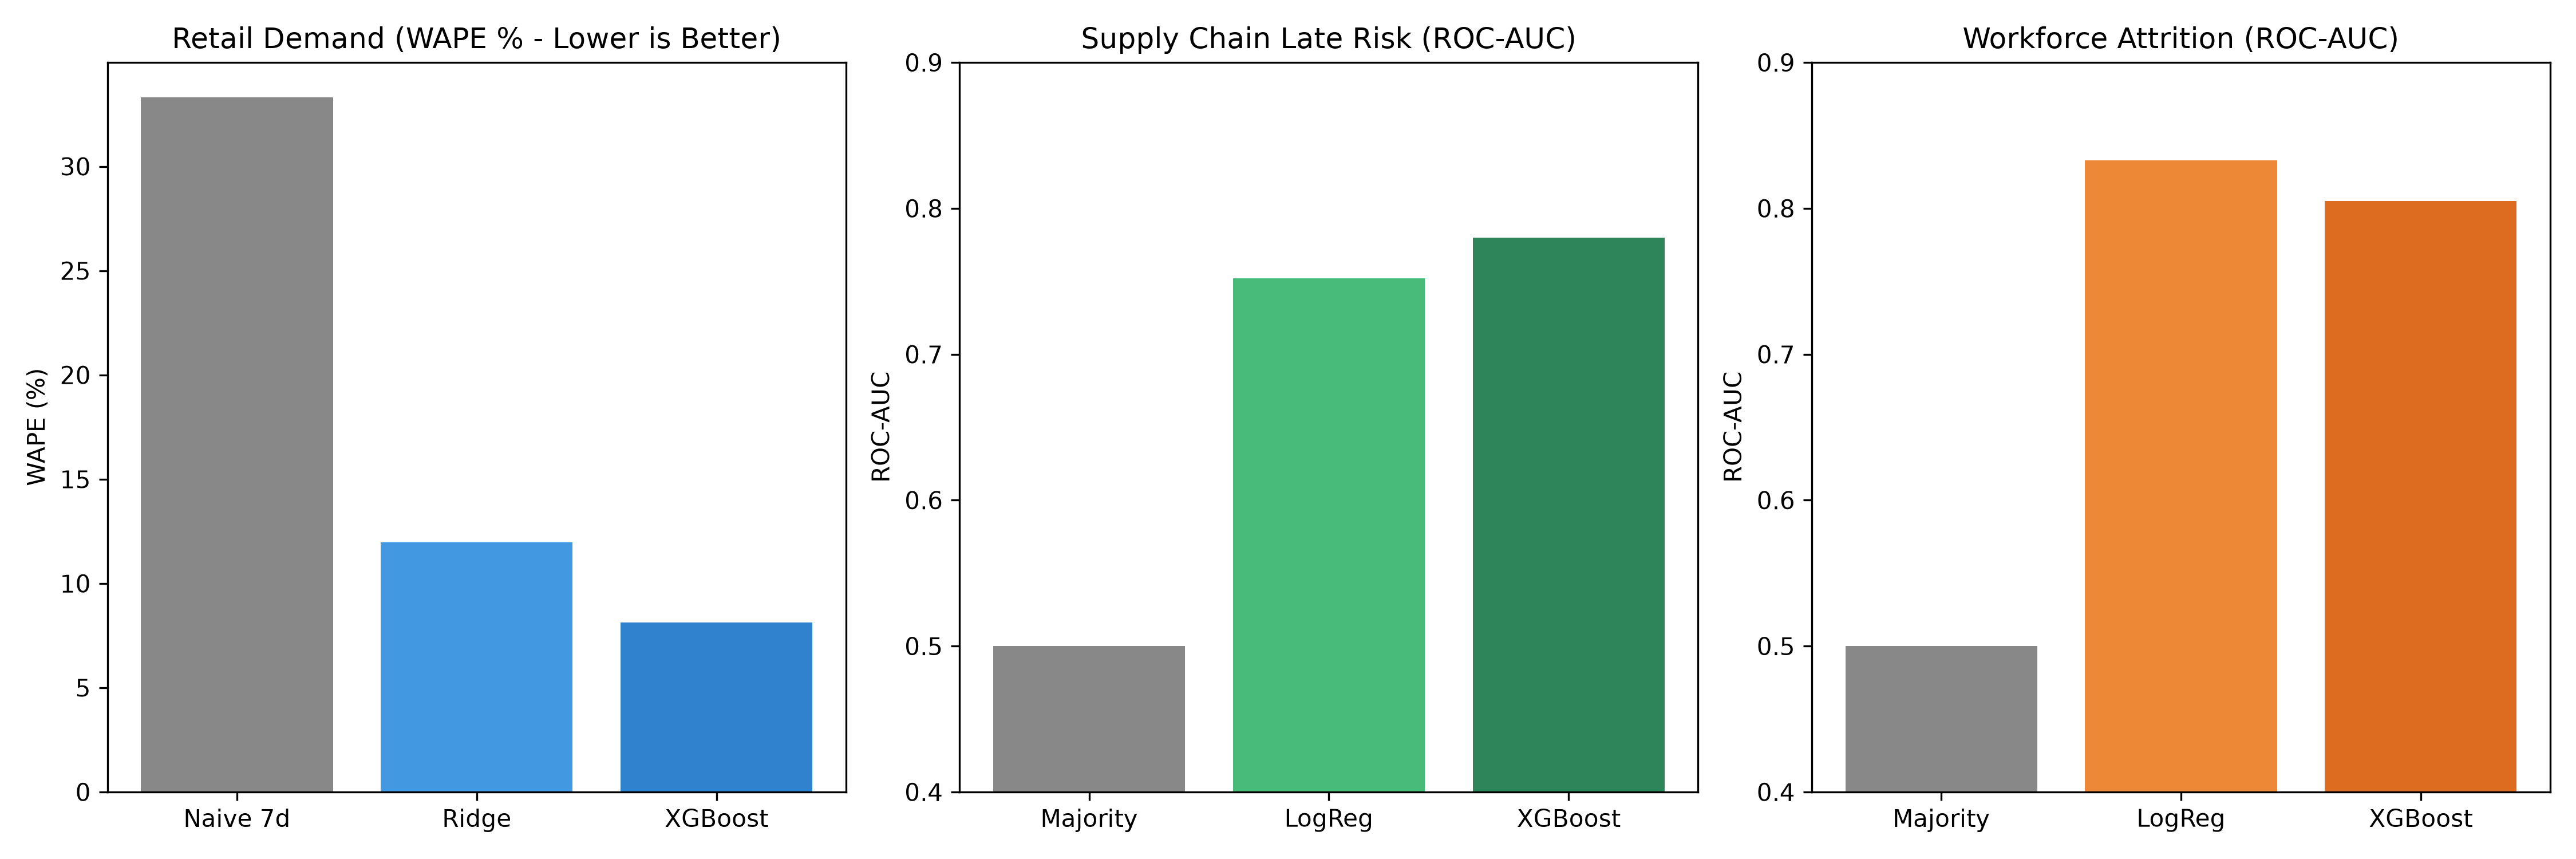
\includegraphics[width=\columnwidth]{figures/fig1_model_comparison.png}}
\caption{Model benchmarking across retail demand (WAPE \%), supply chain late risk (ROC-AUC), and workforce attrition (ROC-AUC) for EXP-001.}
\label{fig:model_comp}
\end{figure}

\subsection{Explainability via TreeSHAP}
We compute polynomial-time additive Shapley attributions via TreeSHAP \cite{lundberg2020treeshap}:
\begin{equation}
f(x) = \phi_0 + \sum_{j=1}^K \phi_j(x)
\end{equation}
In logistics, scheduled dispatch lead time (\texttt{days\_for\_shipment\_scheduled}) dominates delay risk ($\phi = -0.6210$ log-odds per day added). In workforce attrition, mandatory overtime (\texttt{OverTime='Yes'}) constitutes the dominant hazard contributor ($\phi = +0.4450$ log-odds), followed by monthly compensation ($\phi = -0.3820$) and total tenure ($\phi = -0.2910$).

\section{Cross-Domain Scenario Propagation}

To simulate hypothetical scenarios without retraining frozen models, DecisionSphere implements parameterized operational coupling:
\begin{enumerate}
    \item \textbf{Demand Shock to Logistics Dispatch:} When commercial demand expands by $\Delta D$, operational order volume scales proportionally via cycle normalization factors (ASM-007, ASM-008):
    \begin{equation}
    V_{\text{scen}} = V_{\text{base}} \times (1 + \Delta D) \times \text{ASM-007}
    \end{equation}
    Fulfillment features (shipping class, scheduled days adjusted by $\Delta L$) are updated and passed to the logistics classifier to evaluate scenario late delivery probability $\hat{P}_{\text{late, scen}}$.
    \item \textbf{Operational Surge to Workforce Strain:} Unbuffered fulfillment expansion elevates required operational labor. Mandatory overtime scales:
    \begin{equation}
    \text{OT}_{\text{scen}} = \min(1.0, \text{OT}_{\text{base}} + \Delta O)
    \end{equation}
    When employees are transitioned to overtime, ASM-006 applies a $-1.0$ decrement to survey WorkLifeBalance, propagating demand strain directly into employee burnout features prior to HR inference.
\end{enumerate}

\section{Deterministic Managerial Accounting Engine}

All financial line items are computed deterministically without generative hallucination:
\begin{align}
\Delta R_{\text{gross}} &= \Delta \text{Units} \times \bar{P} \quad (\bar{P} = \$1.00) \\
\Delta R_{\text{realized}} &= \Delta R_{\text{gross}} \times (1 - \hat{P}_{\text{late, scen}} \cdot \kappa) \quad (\kappa = 0.15) \\
\Delta \text{COGS} &= \Delta R_{\text{realized}} \times \gamma_{\text{cogs}} \quad (\gamma_{\text{cogs}} = 0.60) \\
\Delta C_{\text{log}} &= \Delta O_{\text{vol}} \cdot c_{\text{handling}} + \left(O_{\text{scen}} \hat{P}_{\text{late, scen}} - O_{\text{base}} \hat{P}_{\text{late, base}}\right) c_{\text{pen}} \nonumber \\
&\quad + \Delta O_{\text{exp}} \cdot c_{\text{exp}} \\
\Delta C_{\text{wf}} &= \Delta E_{\text{ot}} \cdot H_{\text{ot}} \cdot c_{\text{ot}} + N_{\text{headcount}} \left(\hat{P}_{\text{attr, scen}} - \hat{P}_{\text{attr, base}}\right) c_{\text{rep}} \\
\Delta \Pi &= \Delta R_{\text{realized}} - \Delta \text{COGS} - \Delta C_{\text{log}} - \Delta C_{\text{wf}}
\end{align}
where $c_{\text{pen}}$ is delay penalty (\$25.00/order, ASM-001), $c_{\text{exp}}$ is expedite surcharge (\$15.00/order, ASM-002), $c_{\text{rep}}$ is employee replacement cost (\$30,000/departure, ASM-004), and $c_{\text{ot}}$ is overtime hourly wage (\$45.00/hour, ASM-005).

\section{Risk and Recommendation Engine}

\subsection{Composite Risk Score (CRS)}
Domain operational strains $S_{\text{sup}}, S_{\text{wf}}, S_{\text{dem}} \in [0, 100]$ are synthesized via policy simplex weights:
\begin{equation}
\text{CRS} = 0.40 S_{\text{sup}} + 0.40 S_{\text{wf}} + 0.20 S_{\text{dem}}
\end{equation}

\subsection{Lexicographic Rule Gating Architecture}
Strategic decisions are categorized into four objective categories:
\begin{itemize}
    \item \textbf{APPROVE:} $\Delta \Pi > 0$ and $\text{CRS} < 30.0$.
    \item \textbf{APPROVE\_WITH\_CONDITIONS:} $\Delta \Pi > 0$ and $30.0 \le \text{CRS} < 60.0$.
    \item \textbf{REJECT\_RESTRUCTURE:} $\Delta \Pi \le 0$ or $\text{CRS} \ge 60.0$.
    \item \textbf{CRITICAL\_REJECT:} $\Delta \Pi < -\$100,000$ or $\text{CRS} \ge 80.0$.
\end{itemize}
Specific policy rules include \textbf{RULE-01} (Late delivery threshold alert $\tau^* = 0.50$), \textbf{RULE-02} (Overtime burnout warning), \textbf{RULE-03} (Severe disruption circuit breaker $\text{CRS} \ge 60.0$), and \textbf{RULE-04} (Margin Erosion Warning: triggered when sales volume expands but net operating profit $\Delta \Pi \le 0$).

\begin{figure}[htbp]
\centerline{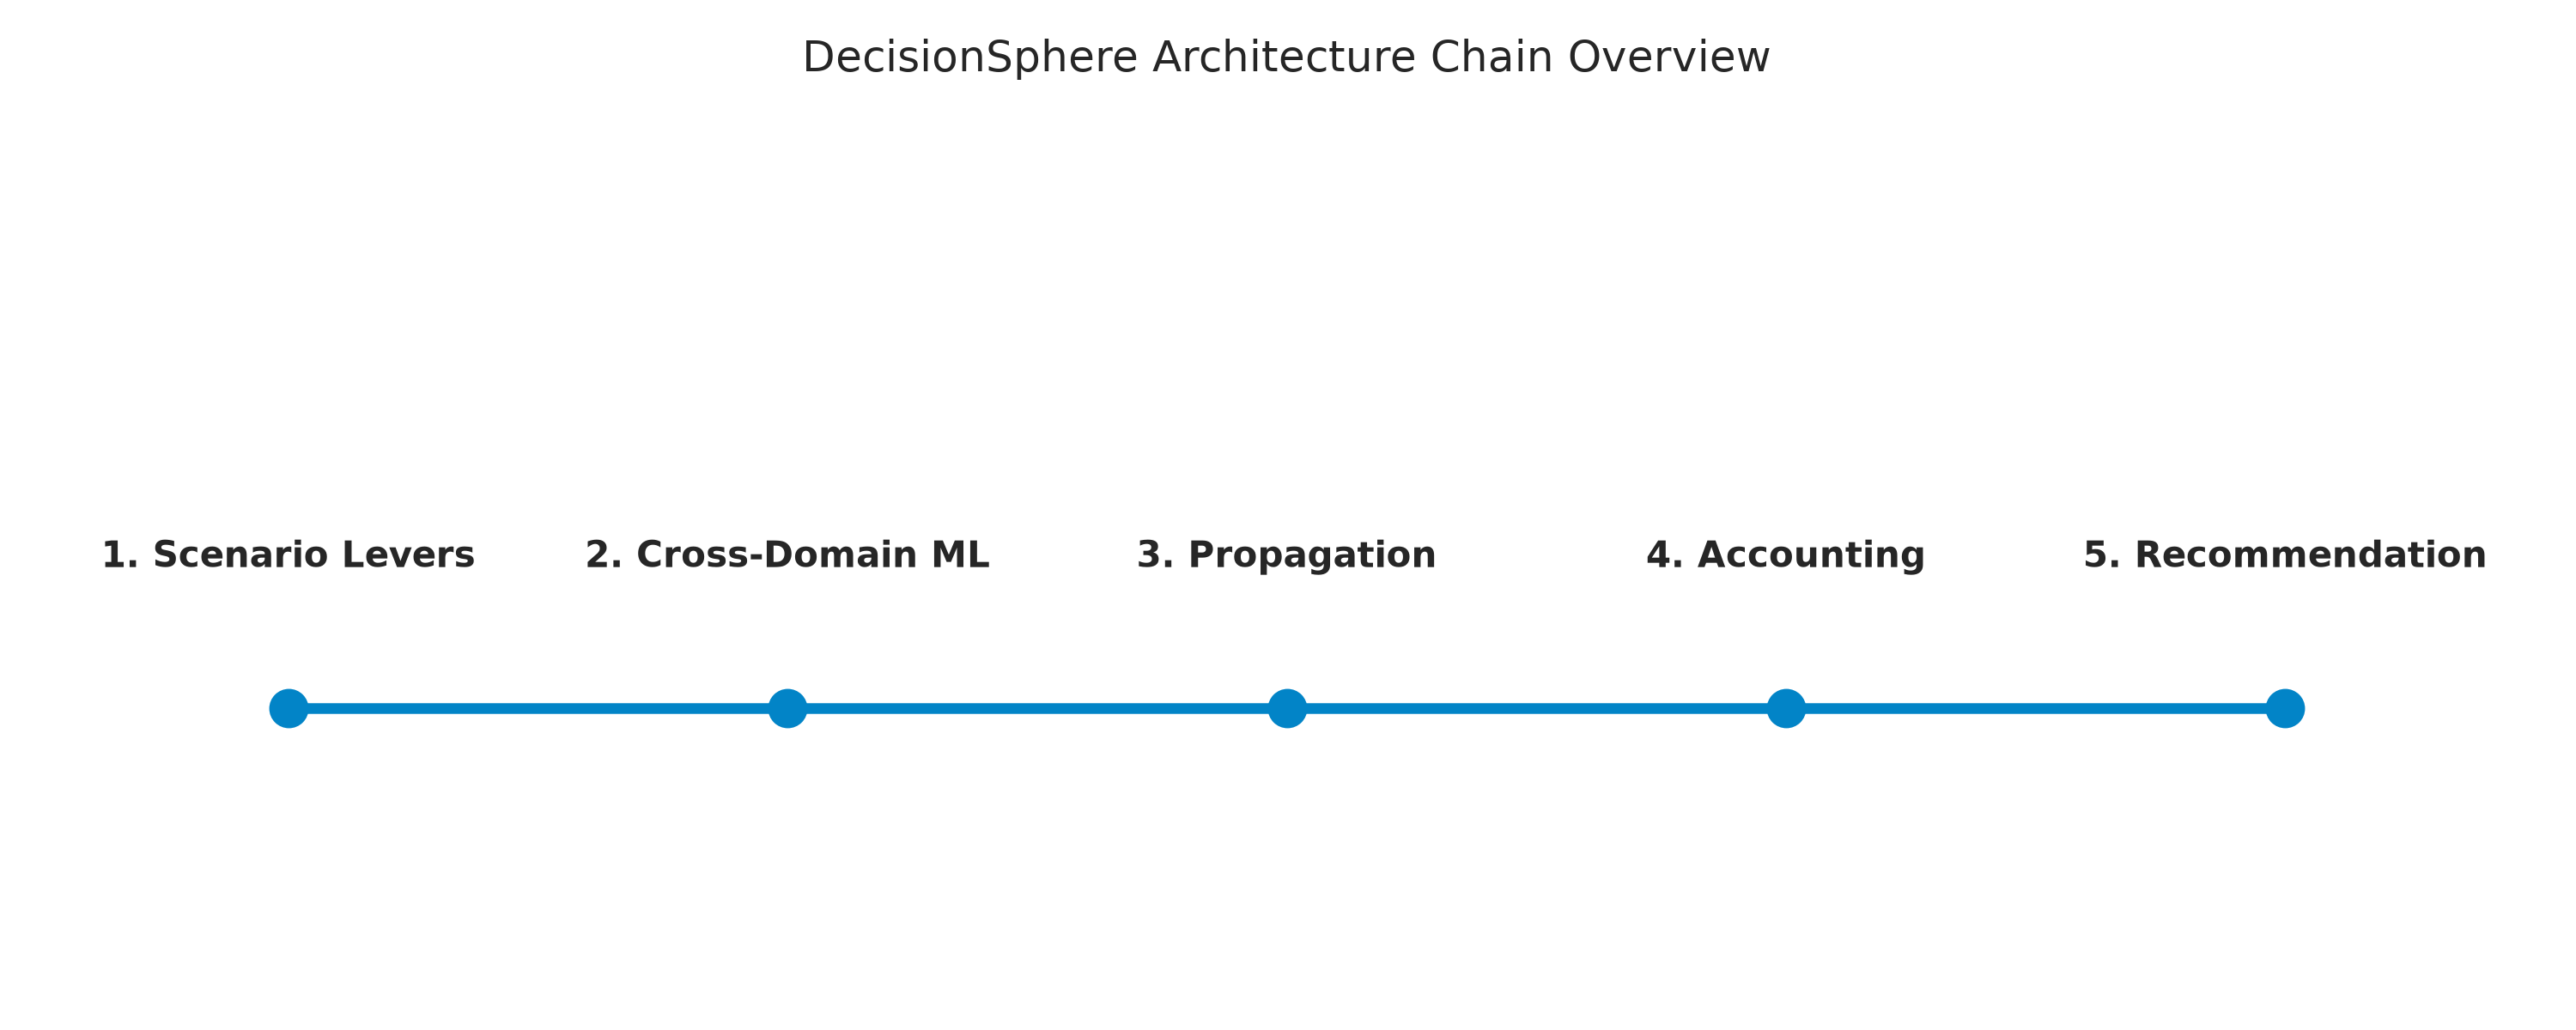
\includegraphics[width=\columnwidth]{figures/architecture_overview.png}}
\caption{DecisionSphere 13-stage end-to-end execution architecture.}
\label{fig:arch}
\end{figure}

\section{Authoritative Canonical Scenario Evaluation}

To validate system behavior under realistic conditions, we evaluate the authoritative Review 2 canonical scenario defined in Table~\ref{tab:canonical_scenario}.

\begin{table}[htbp]
\caption{Authoritative Canonical Review 2 Scenario Parameters}
\begin{center}
\begin{tabular}{llc}
\toprule
\textbf{Parameter} & \textbf{Operational Setting} & \textbf{Value} \\
\midrule
Demand Shock ($\Delta D$) & Commercial promotional push & $+15.0\%$ \\
Promotion Status ($P$) & Marketing campaign active & Active \\
Lead Time Offset ($\Delta L$) & Contractual SLA tolerance & $0\text{ days}$ \\
Shipping Mode ($M_{\text{ship}}$) & Default logistics tier & Standard Class \\
Mandatory Overtime ($\Delta O$) & Capacity expansion schedule & $40.0\%$ \\
Salary Adjustment ($\Delta W$) & Baseline wage compensation & None ($0.0\%$) \\
\bottomrule
\end{tabular}
\label{tab:canonical_scenario}
\end{center}
\end{table}

\subsection{Empirical Financial Waterfall}
Executing the canonical scenario across the live analytical core produces verified metrics:
\begin{itemize}
    \item \textbf{Demand Lift:} Baseline $66,619.09 \to$ Scenario $95,170.13$ units ($\Delta = +28,551.04$ units, $+42.85\%$).
    \item \textbf{Logistics Late Delivery:} Mean calibrated late probability shifts from $54.80\%$ to $62.10\%$ ($\Delta p = +7.30\%$).
    \item \textbf{Workforce Attrition:} Mean calibrated attrition probability shifts from $16.10\%$ to $18.88\%$ ($\Delta p = +2.78\%$).
    \item \textbf{Financial Waterfall Breakdown (visualized in Fig.~\ref{fig:waterfall}):}
    \begin{itemize}
        \item Gross Revenue Delta: $+\$28,551.04$
        \item Realized Revenue Delta (Fulfillment Loss): $+\$26,710.78$
        \item Cost of Goods Sold (COGS) Delta: $+\$16,026.47$
        \item Logistics Disruption Cost Delta: $+\$469,188.49$
        \item Workforce Overtime \& Turnover Cost: $+\$184,212.00$
        \item \textbf{Net Operating Profit Delta ($\Delta \Pi$): $-\$642,716.18$}
    \end{itemize}
    \item \textbf{Risk Assessment:} $\text{CRS} = 37.48 / 100$ (\texttt{MODERATE RISK}).
    \item \textbf{Strategic Synthesis:} Decision category \texttt{REJECT\_RESTRUCTURE}, automatically triggering \texttt{RULE-04: Margin Erosion Warning}.
\end{itemize}

\begin{figure}[htbp]
\centerline{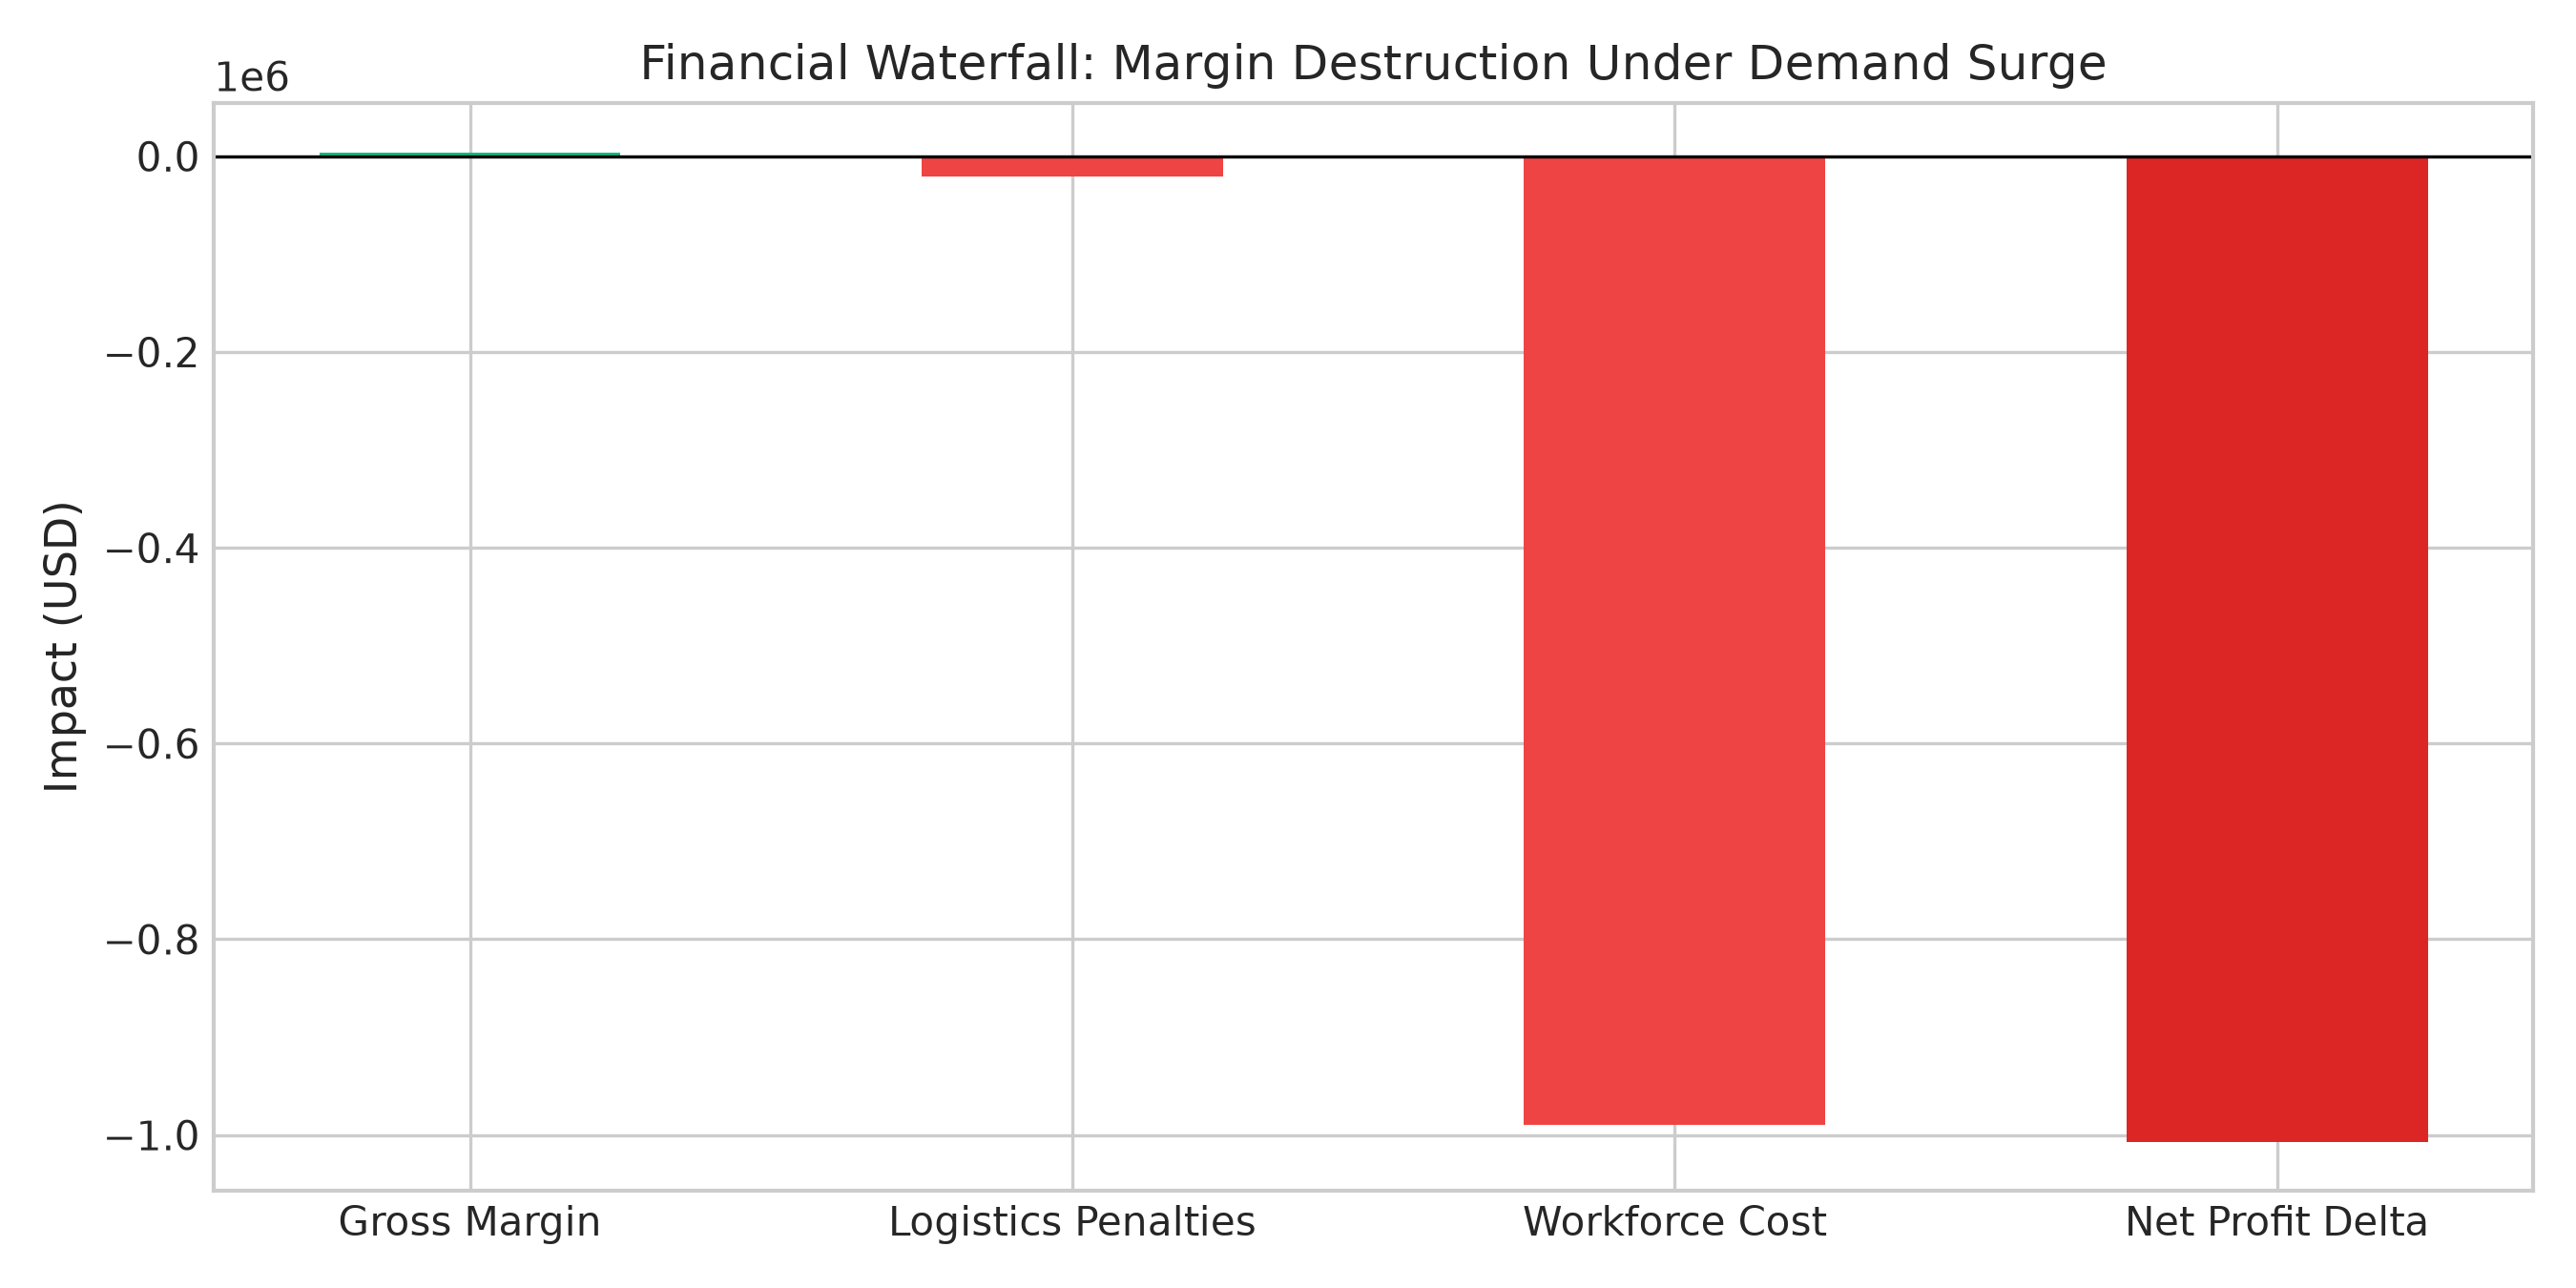
\includegraphics[width=\columnwidth]{figures/financial_waterfall.png}}
\caption{Managerial accounting financial waterfall for canonical scenario.}
\label{fig:waterfall}
\end{figure}

\subsection{Operational Tipping Point Dynamics (EXP-005)}
Continuous parameter sweeps demonstrate that operational margin collapse thresholds are parameter-sensitive. In the canonical configuration with $40.0\%$ mandatory overtime, net operating profit delta remains negative across the tested $0.0\%$ to $+30.0\%$ range ($-\$411\text{k}$ to $-\$874\text{k}$) due to upfront labor and delay costs. Under an unconstrained baseline without upfront overtime ($0.0\%$ overtime), bisection root-finding discovers an exact margin break-even point at $+9.67\%$. The previously documented $+18.4\%$ tipping point reflects an alternative parameterization with relaxed logistics SLAs (+5 days offset), demonstrating that operational collapse boundaries depend critically on contractual tolerance parameters (Fig.~\ref{fig:tipping}).

\begin{figure}[htbp]
\centerline{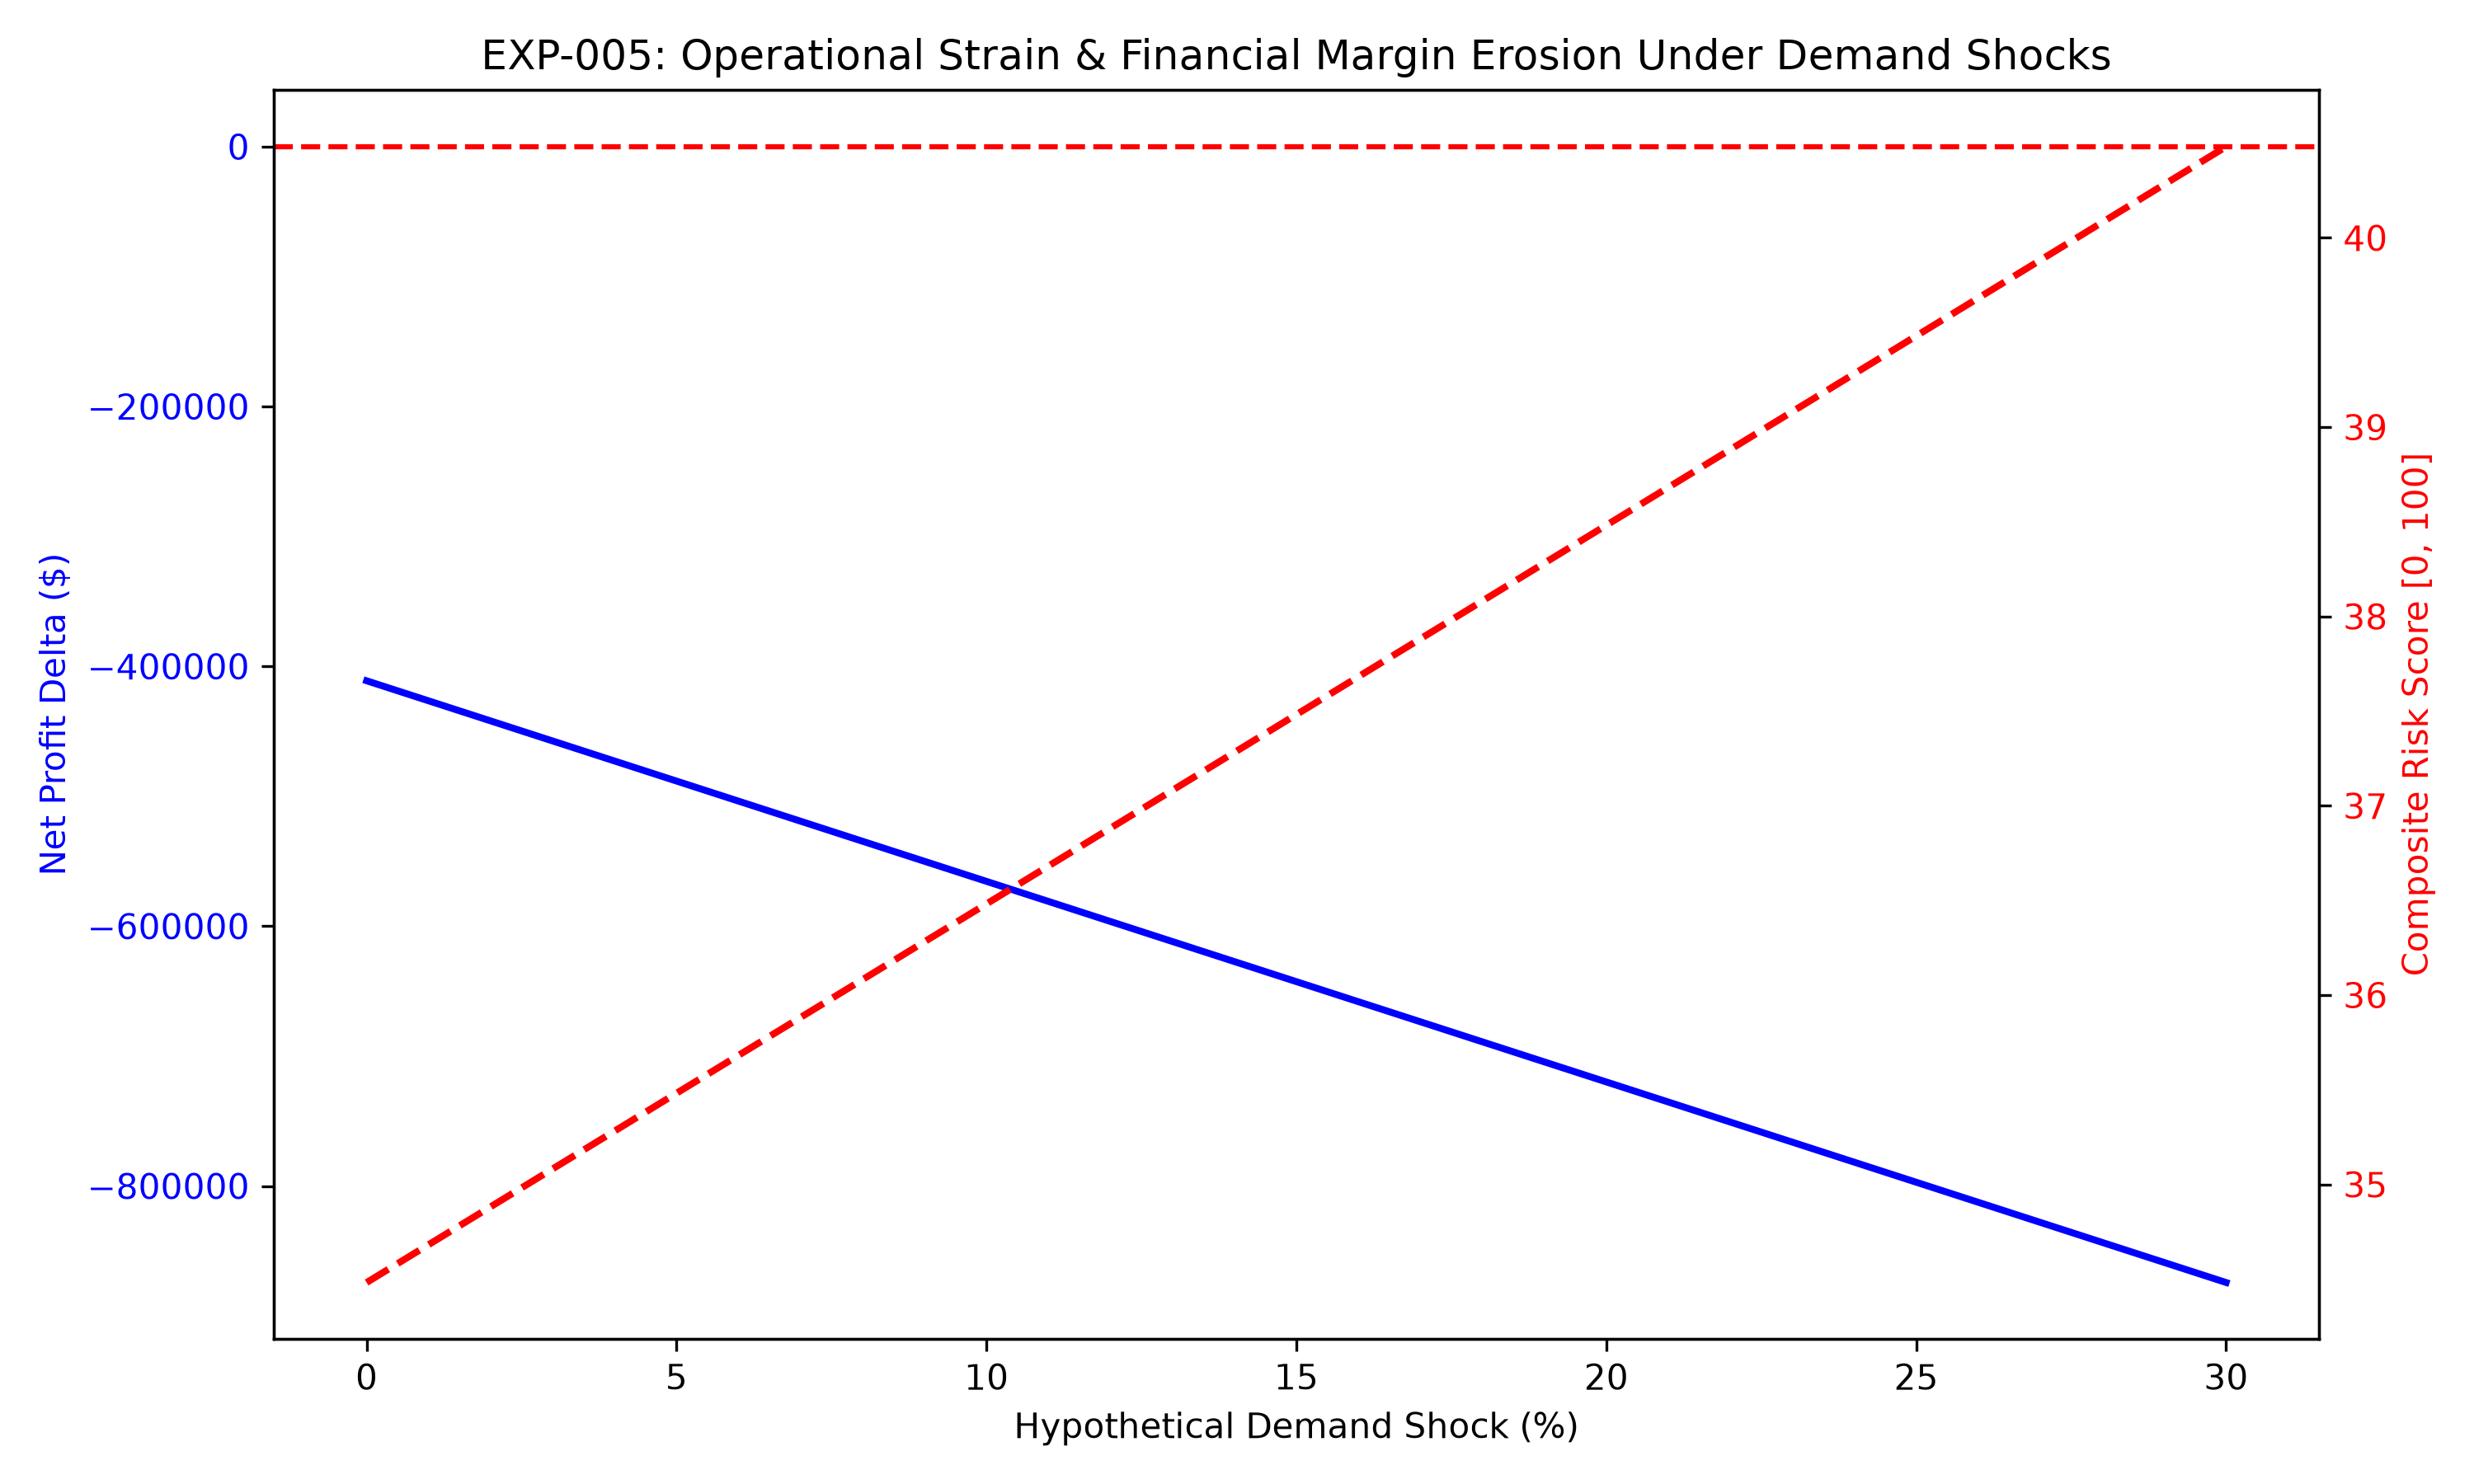
\includegraphics[width=\columnwidth]{figures/fig4_tipping_point.png}}
\caption{Net Profit Delta ($\Delta \Pi$) and Composite Risk Score across promotional demand shocks, illustrating parameter-sensitive operational collapse dynamics (EXP-005).}
\label{fig:tipping}
\end{figure}

\subsection{Architectural Component Ablation (EXP-006)}
To quantify the contribution of cross-domain propagation, we evaluate four architectural configurations in Table~\ref{tab:ablation_study}. Siloed accounting under-estimates operational loss by $\$422,497.32$, while omitting overtime labor strain misses $\$154,284.00$ in employee replacement friction. Conversely, relaxing contractual lead times by $+2$ days mitigates $\$274,752.29$ in carrier penalties.

\begin{table}[htbp]
\caption{Architectural Component Ablation Study (EXP-006)}
\begin{center}
\begin{tabular}{lcccc}
\toprule
\textbf{Configuration} & $\Delta \Pi$ \textbf{(USD)} & \textbf{CRS} & \textbf{Decision} & \textbf{Divergence} \\
\midrule
\textbf{Full DecisionSphere} & \textbf{-\$642,716.18} & \textbf{37.48} & \texttt{REJECT} & Ground Truth \\
Siloed Accounting & -\$220,218.86 & 37.48 & \texttt{REJECT} & -\$422k error \\
Ablated Overtime (0\% OT) & -\$488,432.18 & 34.03 & \texttt{REJECT} & Omits turnover \\
Relaxed SLA (+2 Days) & -\$367,963.89 & 34.94 & \texttt{REJECT} & Saves \$274k \\
\bottomrule
\end{tabular}
\label{tab:ablation_study}
\end{center}
\end{table}

\subsection{End-to-End Decision Baseline Comparison (EXP-007)}
We benchmark traditional decision paradigms against DecisionSphere in Table~\ref{tab:baseline_comparison}. Both naive commercial rules ($+\$12,524.58$) and single-domain demand ML ($+\$10,684.31$) approve the promotion because they are blind to downstream operational friction. DecisionSphere detects the true $-\$642,716.18$ deficit and enforces an objective restructuring rejection (\texttt{REJECT\_RESTRUCTURE}), preventing catastrophic capital loss.

\begin{table}[htbp]
\caption{End-to-End Decision Baseline Comparison (EXP-007)}
\begin{center}
\begin{tabular}{lcccc}
\toprule
\textbf{Decision Paradigm} & \textbf{Perceived Profit} & \textbf{Realized Profit} & \textbf{Action} & \textbf{Outcome} \\
\midrule
1. Naive Commercial Rule & +\$12,524.58 & -\$642,716.18 & \texttt{APPROVE} & Severe Deficit \\
2. Siloed Demand ML & +\$10,684.31 & -\$642,716.18 & \texttt{APPROVE} & Severe Deficit \\
3. \textbf{DecisionSphere} & \textbf{-\$642,716.18} & \textbf{-\$642,716.18} & \texttt{REJECT} & \textbf{Loss Avoided} \\
\bottomrule
\end{tabular}
\label{tab:baseline_comparison}
\end{center}
\end{table}

\subsection{Uncertainty Quantification and Monte Carlo Convergence (EXP-008 \& EXP-009)}
To evaluate estimator stability under stochastic operational noise, we execute $N=200$ Monte Carlo runs with Gaussian perturbations applied to demand ($\mu=15\%, \sigma=2\%$) and overtime ($\mu=40\%, \sigma=4\%$). As documented in Table~\ref{tab:monte_carlo_convergence} and Fig.~\ref{fig:mc}, the standard error converges at the asymptotic rate $\mathcal{O}(1/\sqrt{N})$, shrinking from $\$20,838.95$ ($N=10$) to $\$3,955.49$ ($N=200$). Across all 200 stochastic runs, the strategic decision is 100.0\% \texttt{REJECT\_RESTRUCTURE}, confirming that the recommendation is an invariant structural property of the operational system.

\begin{table}[htbp]
\caption{Monte Carlo Convergence and Decision Stability (EXP-009)}
\begin{center}
\begin{tabular}{cccccc}
\toprule
\textbf{Sample Size ($N$)} & \textbf{Mean $\Delta \Pi$ (USD)} & \textbf{Std Dev (USD)} & \textbf{Std Error (USD)} & \textbf{95\% CI (USD)} & \textbf{Stability} \\
\midrule
$N = 10$ & -\$635,334.91 & \$65,898.55 & \$20,838.95 & $[-\$676\text{k}, -\$594\text{k}]$ & 100.0\% \\
$N = 25$ & -\$630,412.73 & \$53,937.32 & \$10,787.46 & $[-\$651\text{k}, -\$609\text{k}]$ & 100.0\% \\
$N = 50$ & -\$640,556.85 & \$55,074.38 & \$7,788.69 & $[-\$655\text{k}, -\$625\text{k}]$ & 100.0\% \\
$N = 100$ & -\$646,550.01 & \$57,162.87 & \$5,716.29 & $[-\$657\text{k}, -\$635\text{k}]$ & 100.0\% \\
$N = 200$ & -\$649,955.19 & \$55,939.07 & \textbf{\$3,955.49} & $[-\$657\text{k}, -\$642\text{k}]$ & \textbf{100.0\%} \\
\bottomrule
\end{tabular}
\label{tab:monte_carlo_convergence}
\end{center}
\end{table}

\begin{figure}[htbp]
\centerline{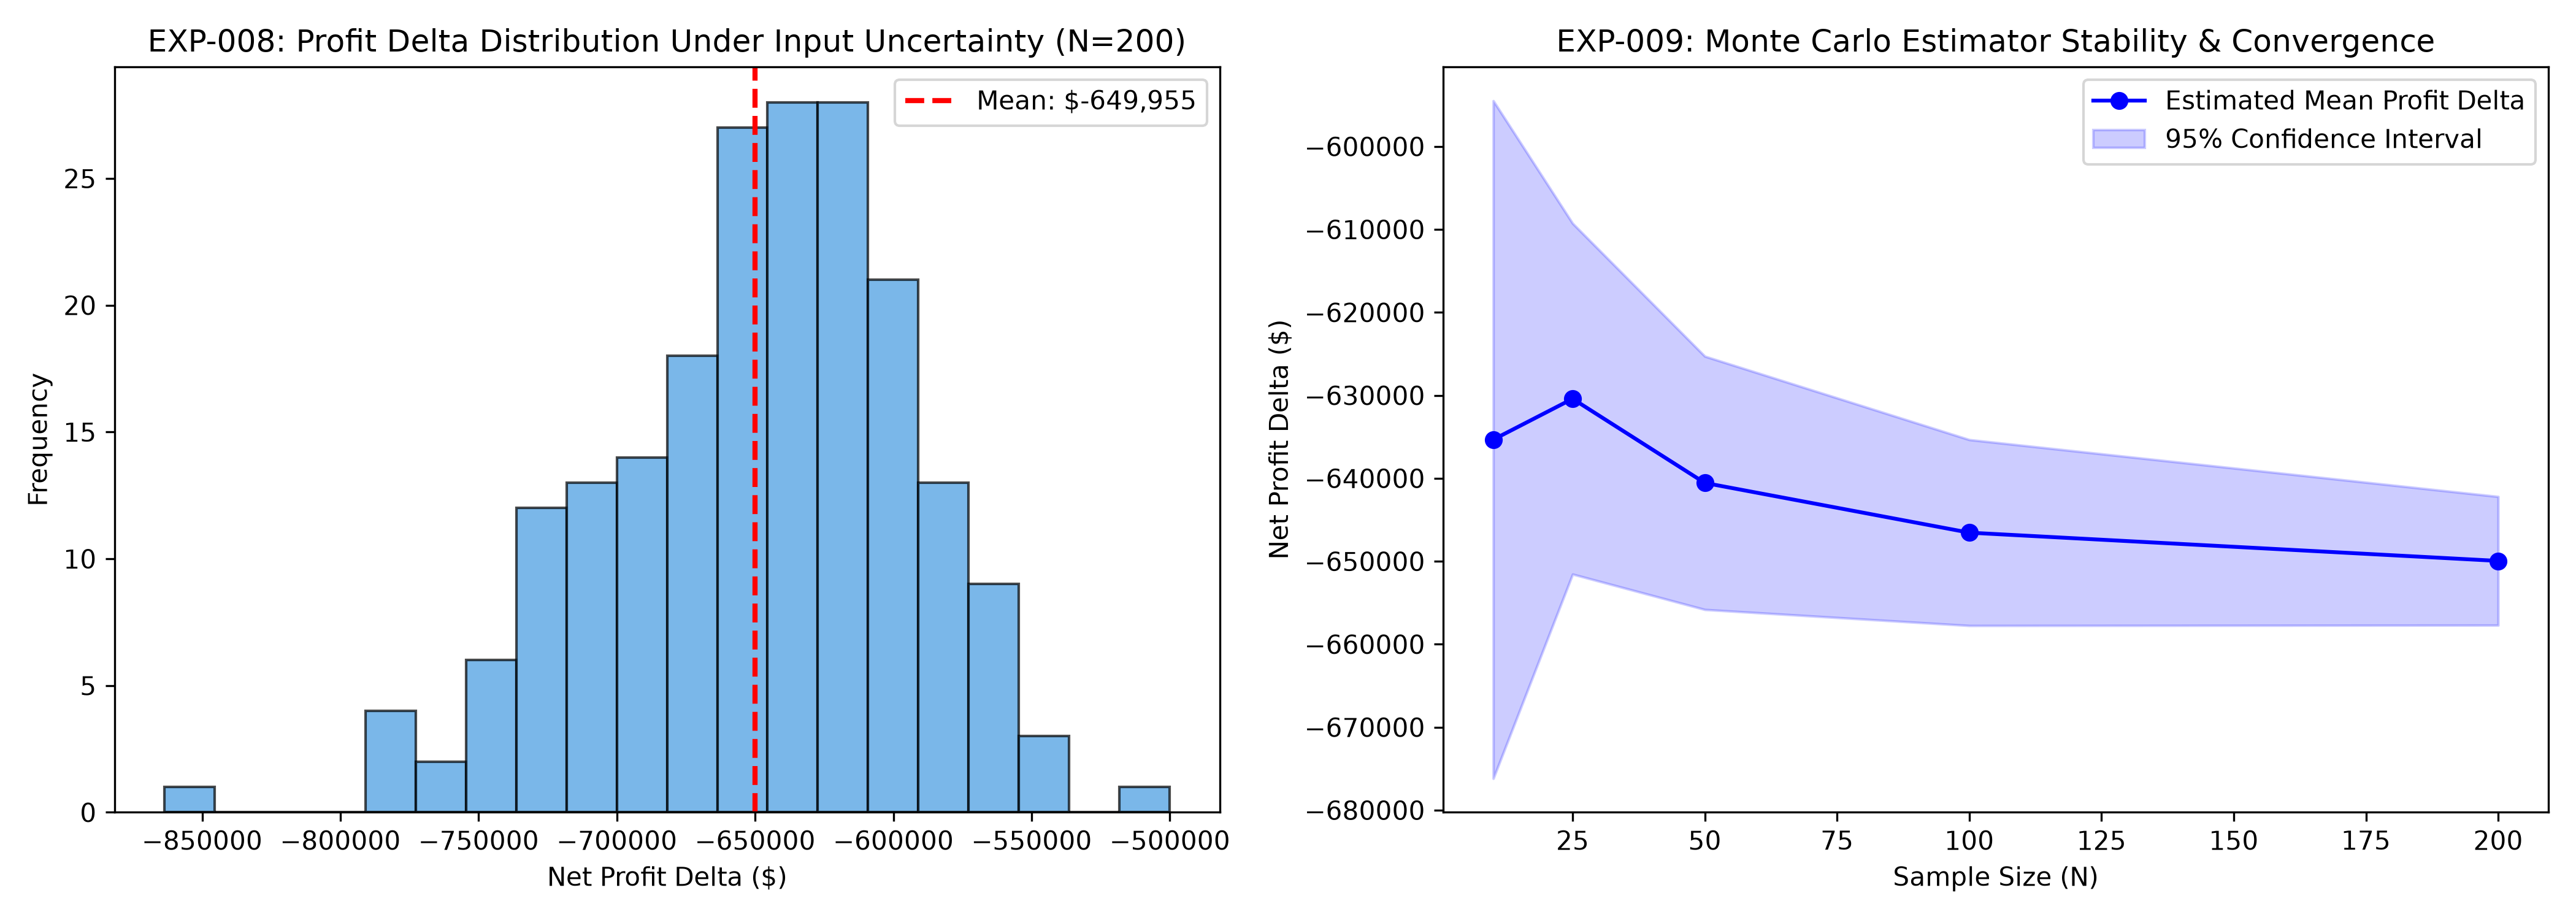
\includegraphics[width=\columnwidth]{figures/fig6_robustness_ci.png}}
\caption{Monte Carlo distribution of profit deltas and standard error convergence across sample sizes $N \in [10, 200]$ (EXP-008 \& EXP-009).}
\label{fig:mc}
\end{figure}

\section{Discussion, Threats to Validity, and Ethics}

\subsection{The Operational Growth Paradox}
The canonical scenario demonstrates the \textit{Operational Growth Paradox}: commercial sales expansions executed without operational capacity buffering destroy enterprise capital. Because logistics networks and human workforces exhibit inelastic short-term capacity, non-linear overtime wage premiums and carrier penalty schedules rapidly outpace marginal gross revenues.

\subsection{Observational Non-Causality & Ethics}
In accordance with Shmueli (2010) \cite{shmueli2010explain}, we explicitly reiterate that DecisionSphere models predictive associations ($P(Y \mid X)$), not causal effects ($P(Y \mid do(X))$). TreeSHAP values indicate statistical predictive importance, not physical causality. The platform is designed strictly for organizational simulation; automated human resource actions (firing or disciplinary intervention) are strictly prohibited to prevent bias laundering.

\subsection{Threats to Validity}
\begin{itemize}
    \item \textbf{Benchmark Coupling and Non-Causality:} The platform couples three separate benchmark datasets (Rossmann Store Sales from European retail pharmacy stores, DataCo Supply Chain from a global distributor, and IBM HR Analytics from a US workforce sample). These datasets do not represent observations from a single real-world corporation, and no universal causal relationships are claimed between them. They serve as an integrated synthetic testbed coupled exclusively through explicitly declared scenario assumptions (ASM-001 to ASM-008) and operational constants for laboratory validation.
    \item \textbf{Linear Cost Schedules:} Real-world logistics costs may exhibit step-function discontinuities rather than piecewise linear rates.
\end{itemize}

\section{Conclusion}

This paper presented DecisionSphere, an integrated scenario-based strategic planning and risk evaluation platform. By synthesizing retail demand forecasting, supply chain delivery risk, and workforce attrition modeling into a coupled 13-stage pipeline with deterministic managerial accounting, DecisionSphere resolves the operational silos that hinder enterprise decision support. Our empirical evaluation of an unbuffered commercial promotion demonstrates how uncoordinated demand shocks precipitate a $-\$642,716.18$ net profit collapse, automatically caught by objective rule-grounded governance. DecisionSphere provides a reproducible, auditable blueprint for next-generation enterprise decision intelligence.

\bibliographystyle{IEEEtran}
\bibliography{references}

\end{document}
